\section{Techniki SHAP i LIME}
Zagadnienia uczenia maszynowego postrzegane są niekiedy jako tzw. czarne skrzynki. Przekonanie to wzięło się z tego że, o ile prostsze modele są łatwo interpretowalne dla człowieka, o tyle te bardziej skomplikowane nie dają już żadnych wskazówek jakie cechy okazały się być decydujące jeśli chodzi o podjęte przez wybrany algorytm decyzje. Z pomocą przychodzą nam techniki SHAP i LIME. Pozwalaja one na przybliżoną ocenę które z cech miały wpływ na wynik klasyfikacji.\\

\subsection{SHAP (SHapley Additive exPlanations)}

\subsection{LIME (Local Interpretable Model-agnostic Explanations)}

Lokalne modele zastępcze to modele interpretowalne, które służą do wyjaśniania pojedynczych przewidywań modeli uczenia maszynowego działających jak "czarne skrzynki". Praca dotycząca lokalnych, agnostycznych względem modelu wyjaśnień interpretowalnych (LIME) proponuje konkretną implementację lokalnych modeli zastępczych. Modele zastępcze są trenowane w celu przybliżenia przewidywań leżącego u podstaw modelu "czarnej skrzynki". Zamiast trenować globalny model zastępczy, LIME skupia się na szkoleniu lokalnych modeli zastępczych, aby wyjaśnić indywidualne przewidywania.\\

Podejście jest dość intuicyjne. Najpierw zapominamy o danych treningowych i wyobrazamy sobie, że mamy tylko model "czarnej skrzynki", do którego możesz wprowadzać dane i otrzymywać przewidywania modelu. Możemy testować skrzynkę tak często, jak chcemy. Naszym celem jest zrozumienie, dlaczego model uczenia maszynowego dokonał pewnego przewidywania. LIME testuje, co dzieje się z przewidywaniami, gdy wprowadzasz do modelu uczenia maszynowego warianty swoich danych. LIME generuje nowy zestaw danych składający się z zakłóconych próbek i odpowiadających im przewidywań modelu "czarnej skrzynki". Na tym nowym zestawie danych a następnie trenuje model interpretowalny, który jest ważony przez bliskość próbek do analizowanego przypadku. Modelem interpretowalnym może być dowolny model z rozdziału o modelach interpretowalnych, na przykład Lasso lub drzewo decyzyjne. Nauczony model powinien być dobrą lokalną aproksymacją przewidywań modelu uczenia maszynowego, ale nie musi być dobrą aproksymacją globalną. Tego rodzaju dokładność nazywa się także lokalną wiernością.\\

Matematycznie, lokalne modele zastępcze z ograniczeniem interpretowalności można wyrazić następująco:\\

\begin{equation}
    {explanation}(x) = \arg\min_{g \in G} L(f, g, \pi_x) + \Omega(g)
\end{equation}

Model wyjaśniający dla instancji \( x \) to model \( g \) (np. model regresji liniowej), który minimalizuje stratę \( L \) (np. błąd średniokwadratowy), mierząc jak blisko wyjaśnienie jest do przewidywania oryginalnego modelu \( f \) (np. model xgboost), przy jednoczesnym zachowaniu niskiej złożoności modelu \( \Omega(g) \) (np. preferowanie mniejszej liczby cech). \( G \) to rodzina możliwych wyjaśnień, na przykład wszystkie możliwe modele regresji liniowej. Miara bliskości \( \pi_x \) definiuje, jak duże sąsiedztwo wokół instancji \( x \) rozważamy dla wyjaśnienia. W praktyce LIME optymalizuje tylko część straty. Użytkownik musi określić złożoność, np. wybierając maksymalną liczbę cech, które może użyć model regresji liniowej. \cite{lime}\\

LIME może być stosowany zarówno dla danych tabelarycznych, obrazów oraz tekstu.\\

\subsection{LIME dla danych tabelarycznych i klasyfikacji wieloklasowej}

Dane tabelaryczne to dane przedstawione w tabelach, gdzie każdy wiersz reprezentuje jedną instancję, a każda kolumna - cechę. Próbki LIME nie są pobierane wokół interesującej instancji, lecz z centralnej masy danych treningowych, co jest problematyczne. Jednakże zwiększa to prawdopodobieństwo, że wynik dla niektórych punktów próbki będzie różnił się od punktu danych, który nas interesuje (instancji), i że LIME będzie w stanie przynajmniej w pewnym stopniu wyjaśnić wynik klasyfikacji.\\

Dane użyte do wyjaśnienia techniką LIME nie powinny być normalizowane czy skalowane. Stanowi to pewnego rodzaju problem gdyż musimy budować nowy model (np. dla naiwnego klasyfikatora Bayesa) aby uniknąć pomyłki z tym bardziej optymalnym już znormalizowanym.\\

Po definicji explainera (w wolnym tłumaczeniu "wyjaśniacza"):

\begin{lstlisting}[caption=Definicja explainera]
#Stworz explainer z danych treningowych (potrzebuje surowych, 
                                         nieprzeskalowanych danych)
explainer = LimeTabularExplainer(
    training\_data=X\_train.values,  # nieprzeskalowane dane treningowe
    feature_names=df.columns[:-1].tolist(),  # nazwy cech
    class\_names=class\_labels,  # nazwy klas
    mode='classification'  # dla zadania klasyfikacji
)
\end{lstlisting}

Następnie wybieramy instancję do interpretacji (najcześciej definiujemy iterator wskazujący na numer instancji w zbiorze testowym) i otrzymujemy graficzne wyjaśnienie podjętej przez algorytm decyzcji:\\

\begin{figure}[H]
    \centering
    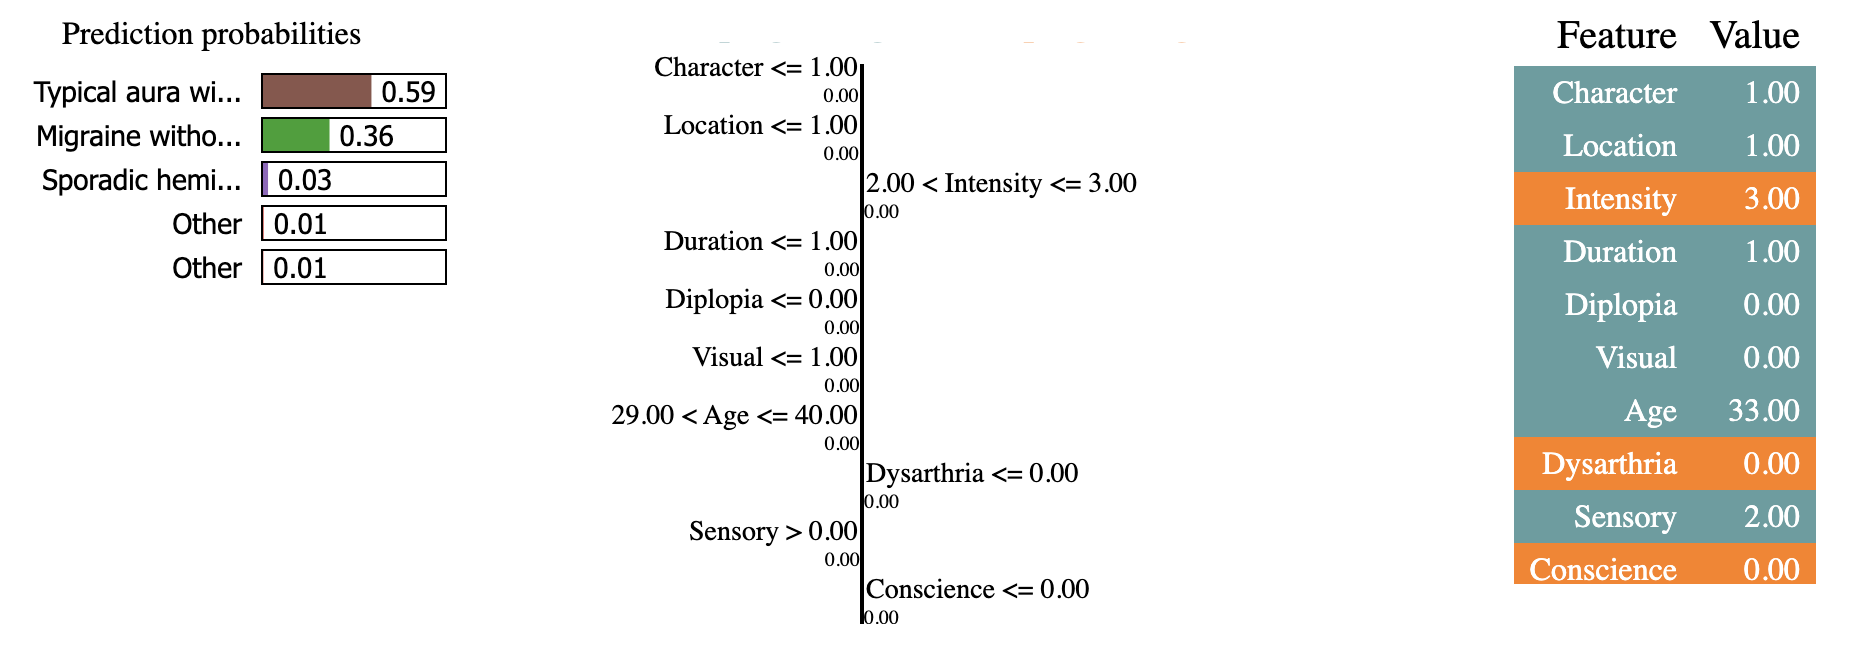
\includegraphics[scale=0.4]{lime_sin}
    \caption{Graficzna interpretacja decyzji modelu}
    \label{fig:lime_sin}
\end{figure}

Po stronie lewej widzimy tabelę podobieństwa do konkretnych klas. Po prawej wartości cech uszeregowane od najistotniejszych wg techniki LIME. Naj widzimy np. Po wartości wiersza "Age" dane nie są skalowane ani normalizowane. Na środku jest najistotniejszy element interpretacji, który akurat w naszym wypadku jest wyjątkowo nieczytelny ze względu na ograniczone możliwości skalowania osi. Natomiast istnieje jeszcze inna możliwość wyświetlenia tego wykresu:\\

\begin{figure}[H]
    \centering
    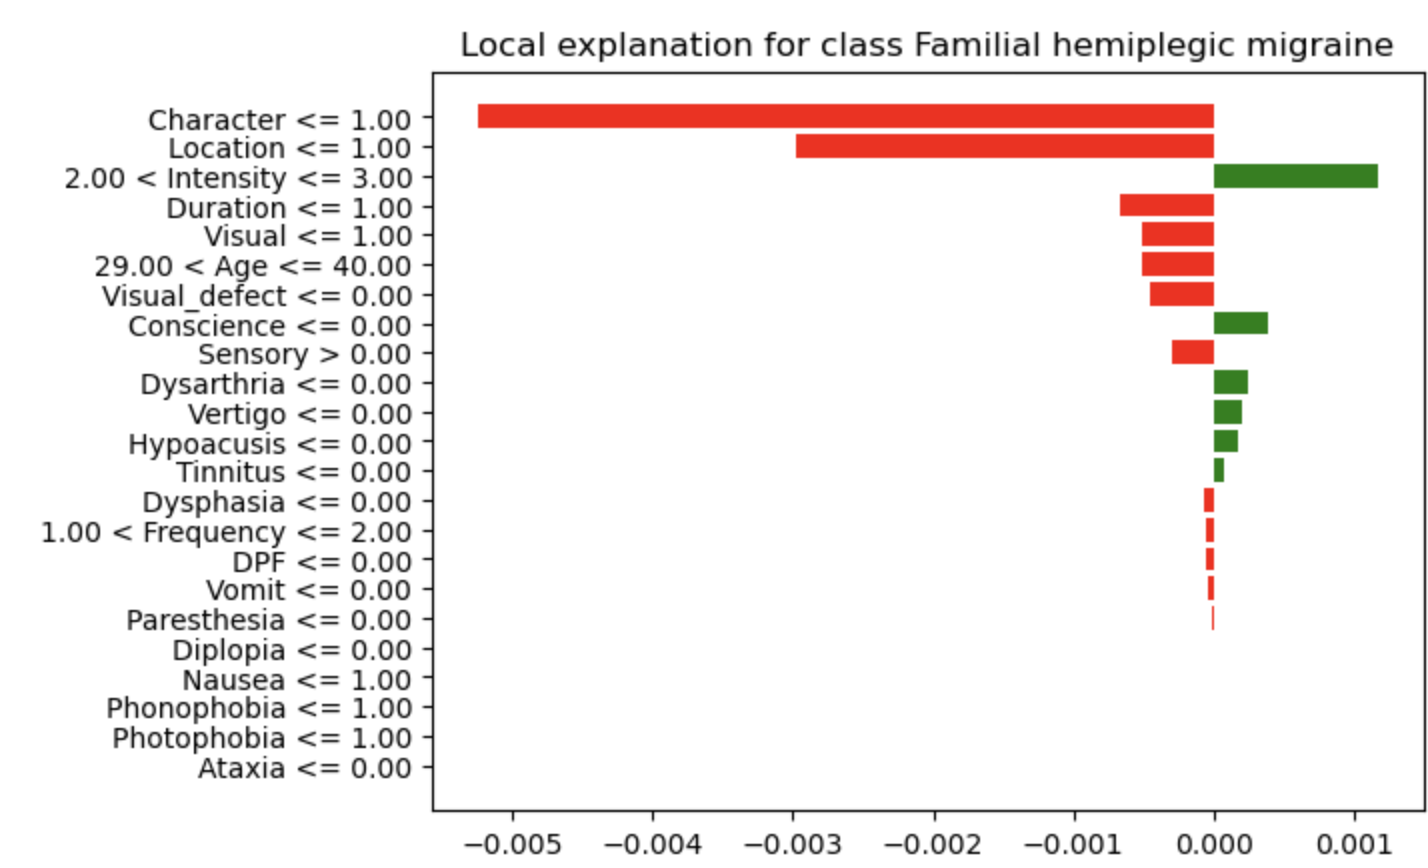
\includegraphics[scale=0.4]{lime_det}
    \caption{Szczegółowy wykres istotności cech}
    \label{fig:lime_det}
\end{figure}

Na osi pionowej widzimy nazwy cech wraz z przedziałami ich wartości dla analizowanej instancji. Na osi poziomej widzimy orientacyjną wartość na cecha ta wpływała na wynik - zarówno jeśli cecha świadczyła za przynależnością do klasy (wartości dodatnie oznaczone na zielono) jak i wpływ cech przeciw klasyfikacji (ujemne wartości oznaczone na czerwono). Dla czytelności wybrałem tabelę z innego przykładu. Widzimy jak pomiędzy obrazkiem nr \ref{fig:lime_det} pokrywają się cechy z lewej i prawej strony osi wobec tego widzimy skróconej interpretacji z obrazka nr \ref{fig:lime_sin}.